\chapter{Software}

Für den Kurs haben wir eine Beispielanwendung, MagicMorph, erstellt.
Ein CMake file bereitgestellt, um Projektdateien für die jeweilige IDE
bzw. ein Makefile zu erzeugen. Die Software basiert
auf OpenGL 3.0 und ist somit auch auf MacOS lauffähig (zwar hat Apple
den Support von OpenGL eingestellt, allerdings werden Anwendungen, welche bis
einschl. maximal Version 4.1 von OpenGL verwenden, nach wie vor unterstützt).
Au\ss erdem nutzen wir folgende externe Bibliotheken:

\begin{itemize}
	\item \textbf{SDL2} als Abstraktion zum Betriebssystem für Fenster und OpenGL-Context Erstellung.
	\\\href{https://github.com/libsdl-org/SDL}{https://github.com/libsdl-org/SDL} 
	\item \textbf{STB image/image write}: Lesen/Schreiben von Bilddateien.
		\\\href{https://github.com/nothings/stb}{https://github.com/nothings/stb} 
	\item \textbf{GLM}: Mathematik Bibliothek, die gut mit OpenGL zusammenarbeitet. 
			\\\href{https://github.com/g-truc/glm}{https://github.com/g-truc/glm}
	\item \textbf{Dear ImGUI}: Immediate Mode GUI Bibliothek für den Editor. 
	\\\href{https://github.com/ocornut/imgui}{https://github.com/ocornut/imgui}
	\item \textbf{tinyfiledialogs}: Betriebssystemunabhängige Bibliothek für Dialogfenster (Nachrichten an Anwender, öffnen, speichern, etc.)	\\\href{https://sourceforge.net/projects/tinyfiledialogs/}{https://sourceforge.net/projects/tinyfiledialogs/}
	\item \textbf{GIF writer von Charlie Tangora}: Speichern der gerenderten Sequenzen als GIF.
				\\\href{https://github.com/charlietangora/gif-h}{https://github.com/charlietangora/gif-h} 
\end{itemize}

\section{Verwenden von MagicMorph}

Die Bedienung ist weitestgehend selbsterklärend. Im \textbf{Source}-Fenster wird eine Linie für ein Feature gezogen. Per
Mausklick wird der Fu\ss punkt der Linie gesetzt, ein weiterer
Mausklick vervollständigt diese. Dabei ist die Richtung der Linie
durch den letzten Klick gegeben. Danach muss
im \textbf{Destination}-Fenster eine weitere Linie erzeugt werden, um das
Paar zu komplettieren. Dieses Vorgehen kann so lange wiederholt
werden, wie gewünscht. Eine bereits gesetzte Linie kann immer mit
der Tastenkombination CTRL+Z rückgängig gemacht werden.
Ist man mit der Definition der Features zufrieden, können mit einem
Klick auf den \textbf{MAGIC!}-Button die Morphs von Quell- und Zielbild
generiert und danach überblendet werden. Je nach Auflösung des Bilderpaares
und der Anzahl gesetzter Linien kann dieser Vorgang ein wenig
dauern. Ist die Berechnung abgeschlossen, so wird ein
neues \textbf{Result}-Fenster geöffnet. Dort lässt sich das
Resultat begutachten. Die Parameter \textbf{a}, \textbf{b} und
\textbf{p}, um das Gewicht einer Linie zu bestimmen, lassen
sich mit den Schiebereglern im \textbf{Control Panel} festlegen.

\begin{figure}[htb]
	\centering
	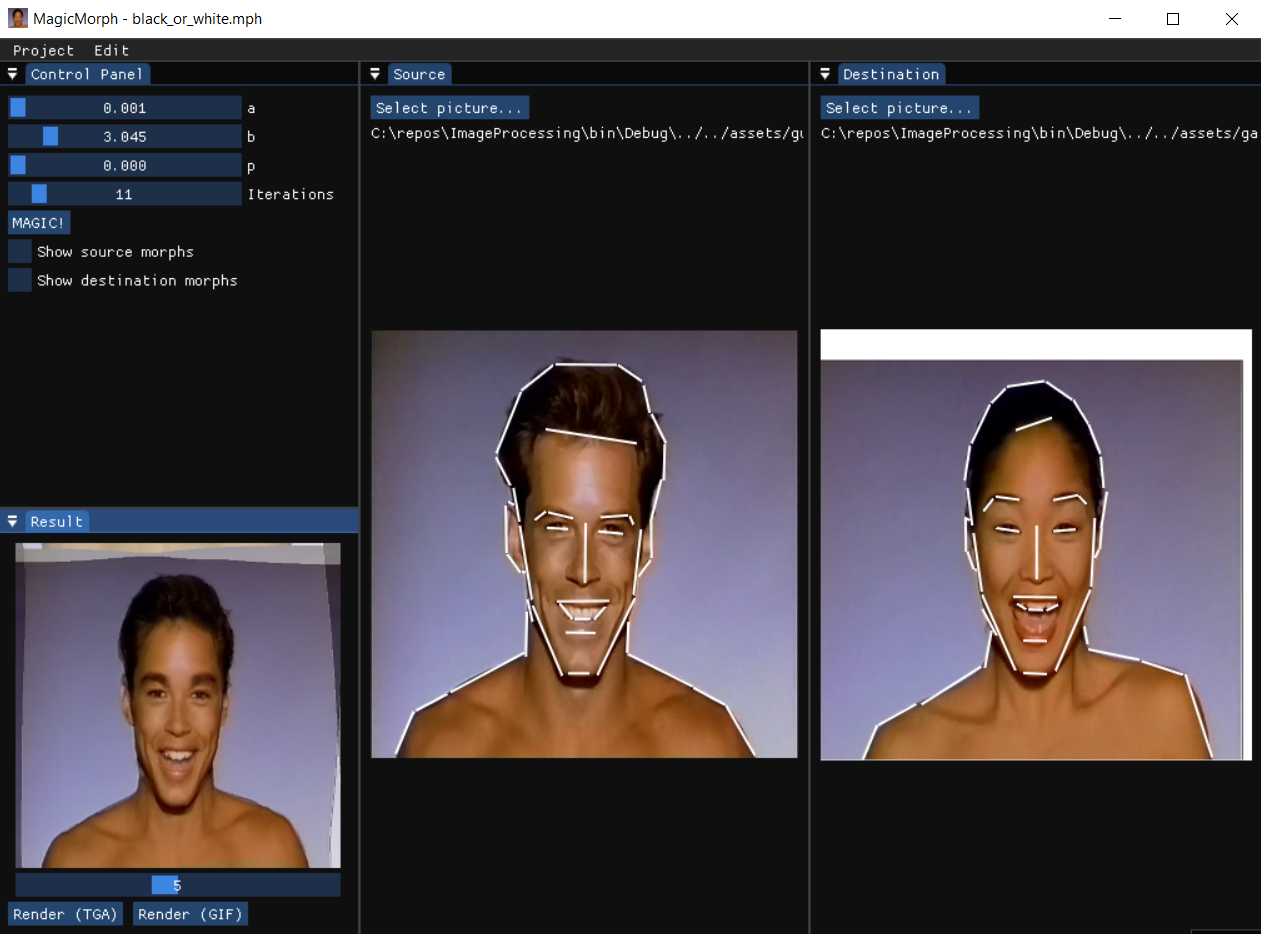
\includegraphics[width=1.0\textwidth]{magicmorph.png}
	\caption{MagicMorph}
	\label{fig:powermorph}
\end{figure}

\section{Ausblick}

Die Interpolation der Linien erfolgt linear für die Start-
und Endpunkte. Wie beschrieben werden Rotationen durch
diese Weise skaliert, auch wenn die Länge des Linienpaares
jeweils gleich bleibt. Beier und Neely beschreiben \cite{beierneely},
dass eine weitere Möglichkeit zur Interpolation folgenderma\ss en
aussieht:
Die Mittelpunkte der beiden Linien und deren Orientierung
werden interpoliert. Darauf wird die Länge der resultierenden
Linie ebenfalls interpoliert. Denkbar wäre hierbei die Nutzung
von Quaternions, welche die Orientierungen der beiden
Linien repräsentieren. Das Erzeugen aus Winkel
und Vektor wird durch \textbf{GLM} unterstützt:

\begin{lstlisting}[language=C++, caption=Quaternions in GLM, label=quaternion, xleftmargin=0.5cm]

glm::quat qSource = glm::angleAxis(theta, glm::vec3(0, 0, 1));
\end{lstlisting}
qSource repräsentiert nun eine Drehung um die Z-Achse
(unsere Linien werden im R2 platziert, wodurch die
3. Dimension hinzugezogen wird, um einen weiteren
Freiheitsgrad zu erlangen).

Den Winkel $\theta$ erhält man durch:

$\theta = \arcsin \left(\frac{y}{\|\textbf{v}\|}\right)$

wobei $y$ die 2. Komponente des Vektors $\textbf{v}$ ist, welcher die Linie in Ziel- bzw. Quellbild repräsentiert.
Die Interpolation zwischen zwei Quaternions erfolgt schlie\ss lich durch:
\begin{lstlisting}[language=C++, caption=Spherical interpolation zwischen zwei Quaternions, label={lst:slerp}, xleftmargin=0.5cm]
	
	glm::quat qInterpolated = glm::slerp(qSource, qDest, 0.5);
	
\end{lstlisting}
In Listing \ref{lst:slerp} wird die Sphärische Interpolation zwischen
zweier Quaternions bei $50\%$ berechnet.
glm::slerp sorgt dafür, dass der kürzeste Pfad zwischen
den beiden Orientierungen genommen wird. Um nun die rotierte (interpolierte)
Linie zu bekommen, wendet man den Quaternion auf die Start- und Endpunkte der
Linie an:
\begin{lstlisting}[language=C++, caption=Rotation der Quelllinie durch einen Quaternion, label={lst:quattimespoint}, xleftmargin=0.5cm]
	
	glm::vec3 aInterpolated = qInterpolated * source.a;
	glm::vec3 bInterpolated = qInterpolated * source.b;
	Line interpolatedLine = Line(
									aInterpolated.x, aInterpolated.y, 
									bInterpolated.x, bInterpolated.y
								 );	
\end{lstlisting}
Nun kann der Pixel $\textbf{X}$ (Pixelposition relativ zur vom Anwender gezogenen Linie) nach $\textbf{X'}$ (Pixelposition relativ zur interpolierten) Linie transformiert werden.



